
\documentclass[12pt]{article}
\usepackage{graphicx}
\usepackage{amsmath}
\usepackage{mathtools}
\usepackage{gensymb}

\newcommand{\mydet}[1]{\ensuremath{\begin{vmatrix}#1\end{vmatrix}}}
\providecommand{\brak}[1]{\ensuremath{\left(#1\right)}}
\providecommand{\norm}[1]{\left\lVert#1\right\rVert}
\newcommand{\solution}{\noindent \textbf{Solution: }}
\newcommand{\myvec}[1]{\ensuremath{\begin{pmatrix}#1\end{pmatrix}}}
\let\vec\mathbf

\begin{document}
\begin{center}
\textbf\large{CHAPTER-11 \\ CIRCLES}

\end{center}
\section*{Excercise 11.1}

Q4.Find the equation of the circle with centre $(1,1)$ and radius $\sqrt{2}$.

\solution
Given
\begin{align}
	\vec{c} = \myvec{1\\1} \text{ and } r = \sqrt{2}
\end{align}
We know the equation of the circle is given as
\begin{align}
	\norm{\vec{x}}^{2} + 2\vec{u}^{\top}\vec{x} + f = 0
\end{align}
So, here
\begin{align}
	\vec{u} &= \myvec{\frac{1}{2}\\[2pt]\frac{1}{2}}\\
	f &= \norm{\vec{u}}^2 - r^2\\
	  &= \myvec{\frac{1}{2}&\frac{1}{2}}\myvec{\frac{1}{2}\\[2pt]\frac{1}{2}}-2\\
	  &=-\frac{3}{2}	  
\end{align}
Thus ,the equation of circle is obtained as
\begin{align}
	\norm{\vec{x}}^2 + \myvec{1&1}\vec{x}-\frac{3}{2} &= 0       		       
\end{align}	
\begin{figure}[!h]
	\begin{center} 
	  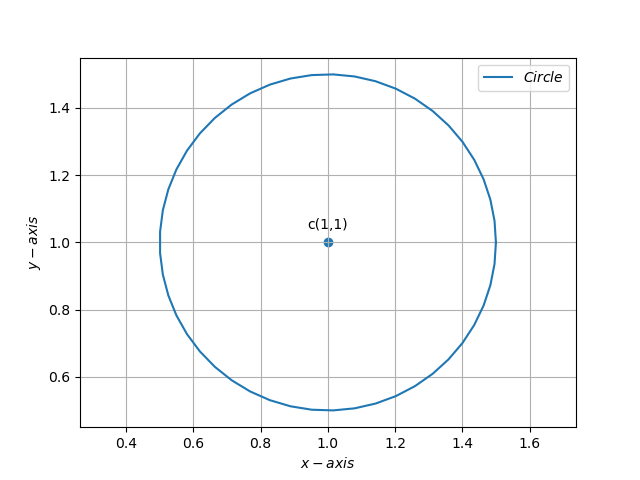
\includegraphics[width=\columnwidth]{/home/srikanth/circle/11.11.1.4/figs/circ.png}
	\end{center}
\caption{}
\label{fig:Fig1}
\end{figure}
\end{document}
